\documentclass{sig-alternate}

\usepackage{amssymb}
\usepackage{amsmath}
\usepackage{graphicx}
\usepackage{epsfig}
\usepackage{subfigure}
\usepackage{listings}
\usepackage{natbib}
\usepackage{verbatim}
\usepackage[T1]{fontenc} 
\usepackage[hyphens]{url}
\lstset{language=ml}
\lstset{commentstyle=\textit}
\lstset{mathescape=true}
\lstset{backgroundcolor=,rulecolor=}
\lstset{frame=single}
\lstset{breaklines=true}
\lstset{basicstyle=\ttfamily}

\pdfpagewidth=8.5in
\pdfpageheight=11in

\begin{document}

\conferenceinfo{SIGITE'11,} {October 20--22, 2011, West Point, New York, USA.} 
\CopyrightYear{2011} 
\crdata{978-1-4503-1017-8/11/10} 
\clubpenalty=10000 
\widowpenalty = 10000

\title{Engaging High School Students in Computer Science via Challenging Applications}

%\begin{comment}
\numberofauthors{4}
\author{
Giuseppe Maggiore \and Andrea Torsello \and Flavio Sartoretto \and Agostino Cortesi \\
       \affaddr{Universit\`a Ca' Foscari Venezia}\\
       \affaddr{Dipartimento di Scienze Ambientali,}\\
       \affaddr{Informatica e Statistica}\\
       \email{\{maggiore, torsello, sartoretto, cortesi\}@dais.unive.it}
}
%\end{comment}

\date{}

\maketitle

\begin{abstract}
In this paper we describe a general framework for building short-courses designed to engage student while presenting a sub-field of computer science. We also describe two of these short-courses centered around computer graphics and physical simulations.

We will discuss how even beginner students can participate in our short-courses; this is possible thanks to a careful choice of development environment, programming language and libraries that allow the students to focus on solving the problems and not thinking about low-level details.
\end{abstract}

\category{K.3.2}{Computers and Education}{Computer and Information Science Education}[Computer science education] 

\terms{Human factors, languages}

\keywords{education, computer science, games}

\section{Introduction}
\label{sec:intro}
%%%%%%%%%%%%%%%%%%%%%%%%%%%%%%%%%%%%%%%%%%%%%%%%%%%%%%%%%%
% intro.tex
%%%%%%%%%%%%%%%%%%%%%%%%%%%%%%%%%%%%%%%%%%%%%%%%%%%%%%%%%%

Game are:
- complex
- require performance

Low-level languages do not cut it fully.

We will:
(A) discuss game constraints
  - discuss traditional approaches and their limitations
  - discuss similarities between game genres and try and find a general framework
  - define a language that is built around this general framework, and which makes it easy
  - reason on why we'd rather have a new language and not just a library
  - give syntax, typing, semantics
(B) give optimization transformations of the language
(C) give a detailed case study
  - give benchmarks that show how effective our optimizations are and how they are completely automated (they require no effort on the part of the programmer) 

\section{A general template}
\label{sec:short-courses_template}
%%%%%%%%%%%%%%%%%%%%%%%%%%%%%%%%%%%%%%%%%%%%%%%%%%%%%%%%%%
% short-courses_template.tex
%%%%%%%%%%%%%%%%%%%%%%%%%%%%%%%%%%%%%%%%%%%%%%%%%%%%%%%%%%

In this section we discuss the general template around which we have structured our short-courses. Before presenting the template, though, we must briefly discuss the purpose of our initiative; in particular, our goals are:
\begin{itemize}
\item interesting students with engaging applications, not just theory
\item showing students real CS tools and techniques for solving actual problems
\item simplifying the problems (to make them solvable in a short time) but without dumbing them down; we *must not* give the impression that CS deals with trivial matters and is somewhat ``inferior'' to maths or engineering
\end{itemize}

Our template for short-courses requires following these steps:
\begin{enumerate}
\item we choose a concrete field of research or application, such as computer graphics, physics simulations, artificial intelligence, security, computer vision, and many others. Any field which has at least one interesting practical application is suitable for our framework;
\item we pick an aspect that is relevant to the field; this aspect can be anything from the accuracy of the simulation to the security of a computer network to the ``smartness'' of an AI, etc. as long as it is easy to visually compare different solutions to see which one is better;
\item we pick a sequence of algorithms, equations or techniques that are designed to improve the parameter (2) with various degrees of complexity and quality of the solution. Ideally, this sequence should be a chain where each algorithm improves the  previous one by adding some complexity, that is each step should be strongly linked to its predecessor and successor;
\item we build a framework which hides all the implementation details that are not strictly relevant to building the various algorithms of (3); this framework should also implement the visualization system. The framework must be built so that the various algorithms of (3) can be plugged in it by the students, if possible even more than one at a time to directly compare them
\item we build the first algorithm of (3) in our system and we document it fully to offer a working starting point to the students
\item we discuss and explain (with a mix of frontal lessons and notes) the underlying theory of the various algorithms of (3) and let the students translate that theory into code that works with the framework (4)
\end{enumerate}

The choice of the actual tools used to implement this template is an important one. There are many valid alternatives, but we believe that the environment used must fulfill the following requirements:
\begin{itemize}
\item it must support advanced rendering and visualization
\item it must support syntactically simple programming languages
\item it should offer auto-completion and helpful error messages (a need eloquently motivated by \cite{SICSC})
\end{itemize}

We have used Microsoft Visual Studio 2010 \cite{VISUAL_STUDIO} with F\# \cite{F_SHARP} and XNA \cite{XNA}. F\# is a functional programming language that belongs to the .Net framework and which can access an extremely large number of mature libraries that can be used for our purposes; F\# is a dialect of the ML family, one of the three large families of functional languages (the other two being LISP and Haskell). It is important to take notice that functional languages are not a requirement of our template: scripting languages such as LUA or Python could arguably be used given their terseness. XNA is a computer graphics library that allows both high-level coding of games and simulations and which also allows in-depth access to the GPU to implement advanced rendering algorithms. XNA has been used in another experimental teaching initiative, as described in \cite{GAME_PROG_FACULTY}: we report similar experiences to theirs, namely that XNA is a powerful framework for teaching that allows students to build interactive applications that can be at any point of the spectrum that goes from simple to program to very complex but visually stunning.

Using these powerful tools has a small downside: some time must be taken, before asking students to operate these tools, to learning the bases of the chosen programming language and environment. F\# offers an immediate console which allows students to experiment with the basic language constructs as the instructor explains them, in order to quickly come to terms with the language.
 

\section{Computer graphics}
\label{sec:computer_graphics}
%%%%%%%%%%%%%%%%%%%%%%%%%%%%%%%%%%%%%%%%%%%%%%%%%%%%%%%%%%
% computer_graphics.tex
%%%%%%%%%%%%%%%%%%%%%%%%%%%%%%%%%%%%%%%%%%%%%%%%%%%%%%%%%%

The main objective of the Computer Graphics short-course is to show students how to compute a realistic appearance for some mesh (3D geometry composed of triangles) through shaders that simulate the visual properties of different materials.

The students are given a starting shader, which is a small program that is run by the GPU and which is responsible for computing the position of the vertices of each triangle and for computing the color of each pixel of the various triangles.

The general shape of a shader is the following (PARAMETERS, VERTEX\_SHADER and PIXEL\_SHADER are just place holders for other code):

\begin{lstlisting}
let shader = 
<@@
  PARAMETERS

  VERTEX_SHADER
  
  PIXEL_SHADER
  
  in ()
@@>
\end{lstlisting}

The shader parameters are a set of global variables that are set to the GPU memory and which store properties of the scene such as the position and color of lights, transformation matrices, etc. The simplest parameters for a 3D scene are provided in the initial shader, and are three transformation matrices: 

\begin{lstlisting}
let World         = parameter() : Matrix
let View          = parameter() : Matrix
let Projection    = parameter() : Matrix
\end{lstlisting}

The students are also given a list of all the global variables that are supported by our system.

A vertex shader takes as input a vertex (which stores the position of the vertex plus optional additional attributes such as its color, its normal, etc.) and returns the transformed vertex (which again contains at least the transformed position plus optional additional attributes). The sample vertex shader simply transforms the input position from 3D space to screen space:

\begin{lstlisting}
  let vertex_shader (InputPosition(pos)) =
    let worldPosition = pos * World
    let viewPosition  = worldPosition * 
                        View
    let pos'          = viewPosition * 
                        Projection

    in OutputPosition(pos')
\end{lstlisting}

A pixel shader takes as input a subset of the attributes of a transformed vertex and returns the color of its pixels; the sample pixel shader returns a uniform red color:

\begin{lstlisting}
  let pixel_shader () =
    OutputColor(Vector4(1f,0f,0f,1f)) 
\end{lstlisting}

Running the initial configuration simply draws a red mesh. Starting from this the students add the normal to the vertex shader input and compute first Lambert lighting and then Phong lighting with a specular component. At this point a color texture is added and read with the input texture coordinates found in the vertex shader; by combining the texturing shader and the Phong shader results a shader capable of showing fine details and lighting (Figure 1). At this point the students replace the background texture with a cubemap which gives the illusion of a more detailed background. The final results are obtained by computing the reflected view direction with respect to the normal of the mesh in order to look up the background, thereby giving the illusion of a reflective surface; by perturbing the normals of the surface in an animated fashion the last shader can be used to show a very pleasant-looking reflective water surface (Figure 2).


\section{Physics simulation}
\label{sec:physics_simulation}
%%%%%%%%%%%%%%%%%%%%%%%%%%%%%%%%%%%%%%%%%%%%%%%%%%%%%%%%%%
% physics_simulations.tex
%%%%%%%%%%%%%%%%%%%%%%%%%%%%%%%%%%%%%%%%%%%%%%%%%%%%%%%%%%

The main objective of the Physics Simulation short-course is to show students how to model simple discrete systems such as a bouncing ball.

The students start with an initial definition of two integrators. The first integrator is loaded from a precomputed file, and it offers an accurate simulation of the real behavior of the system. This first integrator acts as a benchmark. The second integrator simulates simple linear motion. An integrator is specified by giving an instance of the \texttt{Integrator} data-type:

\begin{lstlisting}
// ball = velocity, position
type Ball = float * float

// time = total, delta
type Time = float * float

type Integrator = 
  { 
    // initial position of the ball $y_0$
    y0 : float
    // initial velocity of the ball $v_0$
    v0 : float
    // step-integrator function
    update : Time * Ball -> Ball
    // display name
    name : string 
  }
\end{lstlisting}


The simulation environment takes as input a sequence of integrators to display side-by-side for comparison; the initial sequence the students have is composed of an instance of the precomputed integrator together with the simple linear motion integrator:

\begin{lstlisting}
let actual = { y0 = FromFile.y0; 
              v0 = FromFile.v0; 
              update = FromFile.step; 
              name = "Exact" }
let linear = { y0 = Linear.y0; 
              v0 = Linear.v0; 
              update = Linear.step; 
              name = "Linear1" }

let integrators = 
 seq{
   yield actual
   yield linear
 }
\end{lstlisting}

The students can inspect and modify the code from the linear integrator, which is:

\begin{lstlisting}
let y0 = 10.0
let v0 = 15.0

let step ((t,h),(v,y)) = (v,y + v * h)
\end{lstlisting}

In particular from this integrator the students can see that the \texttt{step} function takes as input the current time \texttt{t}, the step length \texttt{h}, the ball velocity and position \texttt{(v,y)} at time \texttt{t} and returns the new velocity and position of the ball at time \texttt{t+h}.

Running the initial configuration clearly shows that the linear integrator is not an accurate simulation of the benchmark. The students then build a forward Euler integrator which is accurate only during the first seconds of the simulation and which soon starts diverging. They soon realize that the problem is that such a simple, intuitive integrator suffers from unsightly infinite oscillations (the so called \textit{Zeno phenomenon}). Such oscillatory phenomena can be tamed (but never fully corrected) by either cutting the velocity after a while or when they become too small (a very ad-hoc solution) or by using a more refined integrator which suffers from much smaller oscillations. By implementing the Ralston integrator (also known as Second Order Runge-Kutta integrator) the simulation starts to look very accurate (indeed errors and oscillations are smaller than one pixel and cannot be perceived with the naked eye, as seen in the video linked at Figure 3).


\section{Feedback and results}
\label{sec:feedback_and_results}
%%%%%%%%%%%%%%%%%%%%%%%%%%%%%%%%%%%%%%%%%%%%%%%%%%%%%%%%%%
% feedback_and_results.tex
%%%%%%%%%%%%%%%%%%%%%%%%%%%%%%%%%%%%%%%%%%%%%%%%%%%%%%%%%%

We have tried to assess the results of both programs according to the following indicators:

\begin{itemize}
\item perceived satisfaction
\item timely completion of the exercises
\item increase in enrollment
\end{itemize}

Given our original purpose of stimulating interest in Computer Science we are mostly interested in the first item, student satisfaction. Given that we also wished to offer students an active and engaging experience, we also set out to monitor how many students completed our exercises and to what degree. Finally, we wish to monitor the effectiveness of our approach in getting more students enrolled in our degree program.

Unfortunately, we still do not have data about the effectiveness of this year's initiative in terms of student enrollment, given that the next enrollment period has not started yet. We can report as preliminary results the fact that this year we witnessed a small increase in enrollment and we had experimented for the first time with an initiative that was similar to this one (indeed, last year we tried what was the pilot program for this year's initiative). Hopefully this trend will be confirmed in a few months, and in a few years we will have enough data to be of statistical significance.

\paragraph{Computer Graphics}

The computer graphics results have been quite good. As mentioned previously all the students completed their assignments in time. Being the computer graphics assignments both complex \textit{and} time consuming, we were very surprised that all the students managed to work their way through all exercises, even the harder ones. Indeed, we had a ``plan B'' that consisted in showing the correct results after each exercise if too many students had not been able to complete it, in order to level the class so that it could keep moving at a steady pace; such plan was never needed!

The number of students that participated in this course was 31. A questionnaire was created that contained 8 true/false questions about the topics; a few sample questions (we do not include them all for reasons of space) were:

\begin{itemize}
\item ``normals must be transformed into world space before lighting''
\item ``Phong lighting is more accurate than Lambert lighting but is more computationally expensive''
\item ``texture filtering is needed for sampling in-between texels''
\end{itemize}

The resulting error percentages are:

\begin{table}[htb]
\centering
\begin{tabular}{|c|c|c|c|c|c|c|c|}
\hline
Q1 & Q2 & Q3 & Q4 & Q5 & Q6 & Q7 & Q8 \\
\hline
13\% &	0\%	& 7\%	& 3\%	& 7\%	& 3\%	& 7\%	& 20\% \\
\hline
\end{tabular}
\caption{Comprehensions test}
\end{table}

As we can easily see, on average questions scored more than 90\% right answers. The students' perceived satisfaction was measured with another questionnaire, which asked questions about each their experience:

\begin{table}[htb]
\centering
\begin{tabular}{|p{1.2cm}|p{1.2cm}|p{1.2cm}|p{1.2cm}|p{1.2cm}|}
\hline
Glad of having participated & Clarity of teachers & Teaching method & Useful-ness of notions & General satisfaction 		\\
\hline
83\%	& 64\%	& 75\%	& 74\%	& 75\% \\
\hline
\end{tabular}
\caption{Student satisfaction}
\end{table}


Students are very satisfied of having participated in the experience, even though they found the frontal parts of the lesson too hard. In general the results are good, and we believe that by simplifying a bit the exercises and by spending more time on the background (vectors and trigonometry) these scores could become higher. It is interesting to notice that we also received enthusiastic comments from some students, who wrote further feedback such as \textit{An amazing experience: it shows an aspect of Computer Science I did not believe existed}; many students observed that through this kind of course they came to understand that Computer Science is richer and more complex than they believed.


\paragraph{Physics Simulation}

In a manner similar to that used with the computer graphics short-course we have tried assessing the results of the second short-course. In this case we only administered a final questionnaire about the students satisfaction, and not about their understanding of the matters taught. All students completed all their tasks, and in \textit{far less time} than we had anticipated.

11 students participated in this course. They reported their satisfaction as:

\begin{table}[htb]
\centering
\begin{tabular}{|c|c|c|c|c|}
\hline
Interesting & Fun & Engaging & Boring & Uninteresting\\
\hline
82\% & 36\% & 27\% & 0\% & 0\% \\
\hline
\end{tabular}
\caption{General satisfaction}
\end{table}

\begin{table}[htb]
\centering
\begin{tabular}{|p{1.2cm}|p{1.2cm}|p{1.2cm}|p{1.2cm}|p{1.2cm}|}
\hline
Too hard & Hard & Ok & Easy & Too easy \\
\hline
0\% & 9\% & 82\% & 0\% & 0\% \\
\hline
\end{tabular}
\caption{Difficulty}
\end{table}

\begin{table}[htb]
\centering
\begin{tabular}{|p{1.4cm}|p{1.4cm}|p{1.4cm}|p{1.4cm}|}
\hline
New concepts & Concepts I already knew & New way to study concepts I already knew & Nothing new for me \\
\hline
64\% & 0\% & 36\% & 0\% \\
\hline
\end{tabular}
\caption{Novelty}
\end{table}

As we can see, this second course obtained very high ratings. All students described the course as either fun, interesting, engaging; all but one student found the difficulty appropriate (neither too easy nor too hard); finally, all students felt that we taught them something new, either new concepts or new approaches to concepts they knew already.

In addition two students wrote that they really enjoyed the introductory portions which had been somewhat lacking in the computer graphics short-course and that they really liked the opportunity to experiment theoretical concepts in a programming setting.

As a final notice, we wish to express satisfaction from the fact that we were able to teach differential equations without the usual level of students' stress. Differential equations are often considered a benchmark of obscurity, difficulty and boredom, and we are glad we were able to show them as beautiful mathematical concepts which elegantly capture the essence of important real-world phenomena.



\section{Conclusions and future work}
\label{sec:conclusions}
%% Changed by PS, April 4, 2014.

\section{Future work}
\label{sec:future_work}
The Casanova 2 language is capable of implementing usable and quite complex games. The language, while usable, is currently still in development as it misses a few features. In particular, support for multiplayer games is at this moment lacking. We believe that the existing mechanisms for handling time offered by Casanova 2 could be augmented with relatively little effort in order to greatly simplify the hard task of building multiplayer games. This is part of future work, that we are currently engaging in. We are also doing usability studies using students from various disciplines and backgrounds.

The high level view of the game that the Casanova 2 compiler provides can be exploited in order to improve the programmer experience. This means that we could use tools for code analysis (such as abstract interpretation \cite{nielson1999principles} or type system extensions) in order to better understand the game being built, and to help with correctness analysis, performance analysis, or even optimization.


%\subsection{User study}
%We wish to perform an in-depth user study for Casanova 2 to improve usability in the development process. We have already performed a partial (and quite promising) small user study which we will extend and complete.


%We have performed the following test: we gathered a group of students of game programming and a group of students of game design. We gave them a series of Casanova 2 samples, printed on paper. Each student had to guess the functionality of each sample, and sketch a screen-shot. Furthermore, each student also provided some additional feedback on the language.

%The samples were: (\textit{i}) a string of text moved around the screen with the keyboard, (\textit{ii}) a string of text that moves along a predefined path automatically, and (\textit{iii}) an asteroid shooter.

%Eleven (over a total of thirteen) students understood the samples completely, both drawing the screen-shots and explaining the dynamics of the game correctly. Two students were lost on the syntactic differences between Casanova 2 and the more familiar C-like syntax. The direct feedback was mostly centred around a series of common observations, which are reported in Table \ref{students_feedback}. For each observation, the table reports how many times we encountered it.

%\begin{table}[!t]
%% increase table row spacing, adjust to taste
%\renewcommand{\arraystretch}{1.3}
% if using array.sty, it might be a good idea to tweak the value of
% \extrarowheight as needed to properly center the text within the cells

%\caption{Feedback from students}
%\label{students_feedback}
%\centering

%% Some packages, such as MDW tools, offer better commands for making tables
%% than the plain LaTeX2e tabular which is used here.
%\begin{tabular}{|c||c|}
%\hline
%Syntax is unfamiliar at first & 3\\
%\hline
%Syntax is clear & 8\\
%\hline
%Indentation instead of parentheses is a downside & 2\\
%\hline
%List processing with queries is very effective & 1\\
%\hline
%Rules are a good abstraction for games & 2\\
%\hline
%\end{tabular}
%\end{table}

%We also built a significantly bigger sample, which we asked only three students to study. The sample is a checkpoint-based RTS (see Figure \ref{RTS game} for a screenshot). All students correctly identified the game mechanics, and provided some additional feedback. Most of this feedback overlaps with that obtained for the samples, but some new observations emerge. Arguably, some patterns become visible only with larger samples:
%\begin{itemize}
%\item \texttt{wait} and \texttt{when} are very powerful
%\item Multiple rules on the same field are very powerful
%\item Multiple rules on the same field may lead to behaviours that are complex to understand
%\end{itemize}


\section{Conclusions}
\label{sec:conclusions}

Casanova 2, a language specifically designed for building computer games, may offer a solution for the high development costs of games. The goal of Casanova 2 is to reduce the effort and complexities associated with building games. Casanova 2 manages the game world through entities and rules, and offers constructs (wait and yield) to deal with the run-time dynamics. As shown by the benchmarks in Section \ref{sec:evaluation}, we believe that we have taken a significant step towards reaching these goals. In fact, we achieved at the same time very good performance and simplicity, thereby empowering developers with limited resources.  

\label{app:figures}
%%%%%%%%%%%%%%%%%%%%%%%%%%%%%%%%%%%%%%%%%%%%%%%%%%%%%%%%%%
% figures.tex
%%%%%%%%%%%%%%%%%%%%%%%%%%%%%%%%%%%%%%%%%%%%%%%%%%%%%%%%%%



\begin{figure}
\begin{center}
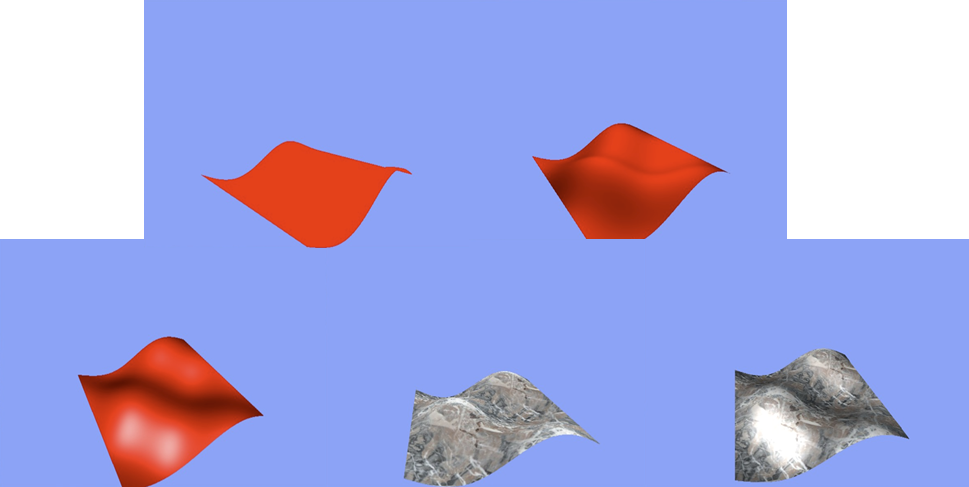
\includegraphics[width=6cm]{uniform_to_texturedphong.png}
\end{center}
\label{uniform_to_texturedphong}
\caption{Uniform Shading, Lambert and Phong Lighting and Texturing}
\end{figure}


\begin{figure}
\begin{center}
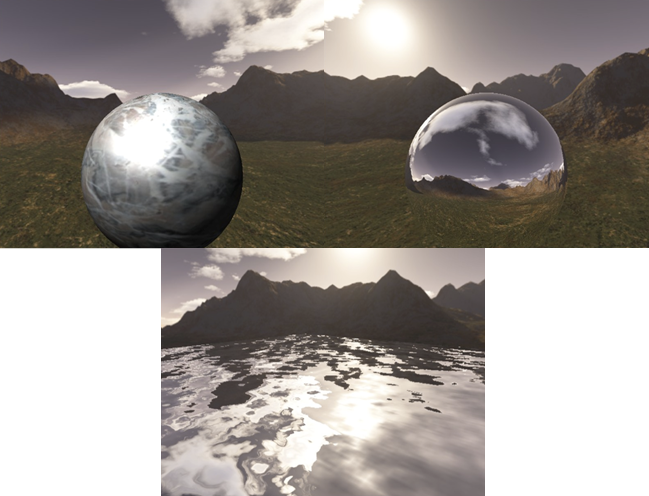
\includegraphics[width=6cm]{reflection_to_water.png}
\end{center}
\label{reflection_to_water}
\caption{Reflection effects}
\end{figure}


\begin{figure}
\begin{center}
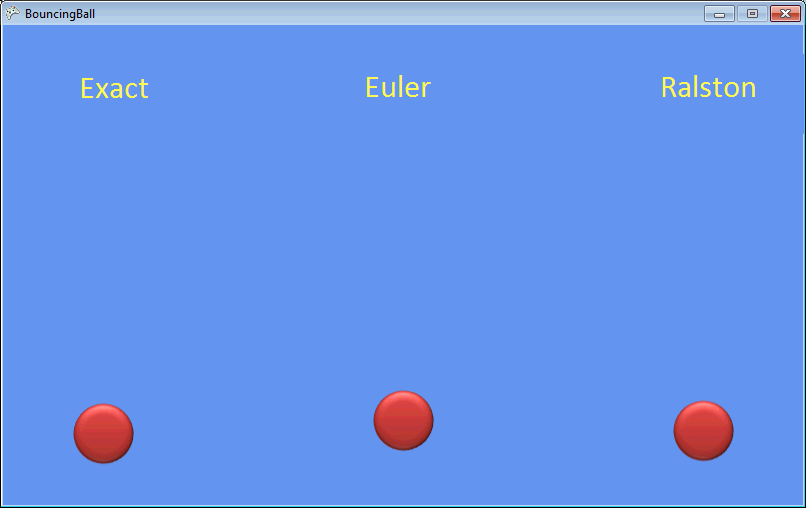
\includegraphics[width=6cm]{ralston.png}
\end{center}
\label{ralston}
\caption{Video found at: http://www.dsi.unive.it/ \~{}orienta/simula/BouncingBall.wmv}
\end{figure} 

\bibliographystyle{plain}
\bibliography{references} 

\nocite{}

\end{document}
